 \documentclass[bachelor, och, labwork]{shiza}
% параметр - тип обучения - одно из значений:
%    spec     - специальность
%    bachelor - бакалавриат (по умолчанию)
%    master   - магистратура
% параметр - форма обучения - одно из значений:
%    och   - очное (по умолчанию)
%    zaoch - заочное
% параметр - тип работы - одно из значений:
%    referat    - реферат
%    coursework - курсовая работа (по умолчанию)
%    diploma    - дипломная работа
%    pract      - отчет по практике
% параметр - включение шрифта
%    times    - включение шрифта Times New Roman (если установлен)
%               по умолчанию выключен
\usepackage{subfigure}
\usepackage{tikz,pgfplots}
\pgfplotsset{compat=1.5}
\usepackage{float}
\usepackage{pdfpages}

\usepackage{titlesec}
\setcounter{secnumdepth}{4}
\titleformat{\paragraph}
{\normalfont\normalsize}{\theparagraph}{1em}{}
\titlespacing*{\paragraph}
{35.5pt}{3.25ex plus 1ex minus .2ex}{1.5ex plus .2ex}

\titleformat{\paragraph}[block]
{\hspace{1.25cm}\normalfont}
{\theparagraph}{1ex}{}
\titlespacing{\paragraph}
{0cm}{2ex plus 1ex minus .2ex}{.4ex plus.2ex}

% --------------------------------------------------------------------------%


\usepackage[T2A]{fontenc}
\usepackage[utf8]{inputenc}
\usepackage{graphicx}
\graphicspath{ {./images/} }
\usepackage{tempora}
\usepackage{kantlipsum}
\usepackage[sort,compress]{cite}
\usepackage{amsmath}
\usepackage{amssymb}
\usepackage{amsthm}
\usepackage{fancyvrb}
\usepackage{listings}
\usepackage{listingsutf8}
\usepackage{longtable}
\usepackage{array}
\usepackage[english,russian]{babel}

%\usepackage[colorlinks=true]{hyperref}
\usepackage{url}

\usepackage{underscore}
\usepackage{setspace}
\usepackage{indentfirst} 
\usepackage{mathtools}
\usepackage{amsfonts}
\usepackage{enumitem}
\usepackage{tikz}

\newcommand{\eqdef}{\stackrel {\rm def}{=}}
\newcommand{\specialcell}[2][c]{%
	\begin{tabular}[#1]{@{}c@{}}#2\end{tabular}}

\renewcommand\theFancyVerbLine{\small\arabic{FancyVerbLine}}

\begin{document}

	\includepdf{yahin-titulnik2.pdf}
	
	%-------------------------------------------------------------------------------------------
	\tableofcontents
	
	\newpage
	
	Цель работы — изучение основных понятий универсальной алгебры и операций над бинарными отношениями. 
	
	\section{Теория}
	    \subsection{Алгебраические операции}

	Отображение $f : A^n \rightarrow A$ называется алгебраической n-арной операцией или просто 
	алгебраической операцией на множестве A. При этом n называется порядком или арностью алгебраической операции $f$.
	
	 Бинарная операция $\cdot$ на множестве A называется:
	
	\begin{enumerate}
		\item ассоциативной, если $\forall x, y, z \in A$ выполняется равенство:	

			$x \cdot (y \cdot z) = (x \cdot y) \cdot z$;
		
		\item коммутативной, если $\forall x, y \in A$ выполняется равенство:		

			$x \cdot y = y \cdot x$;
		
		\item идемпотентной, если $\forall x \in A$ выполняется равенство:
		
			$x \cdot x = x$;

		\item обратимой, если $\forall x, y \in A$ уравнения $x \cdot a = y$ и $b \cdot x = y$  имеют решение, причем единственное;
		
		\item дистрибутивной относительно операции $+$, если $\forall x, y, z \in A$ выполняются равенства
		
			$x \cdot (y + z) = (x \cdot y) + (x \cdot z)$,
			
			$(y + z) \cdot x = (y \cdot x) + (z \cdot x)$;

	\end{enumerate}

\subsection{Основные операции над бинарными отношениями}

\begin{enumerate}
	\item Теоретико-множественные операции ($\cup, \cap, \neg$)
	\item \textit{Обращение} бинарных отношений: обратным для бинарного отношения $\rho \subset A \times B$ называется бинарное
	отношение $\rho^{-1} \subset B \times A$, определяющееся по формуле:

		$\rho^{-1} = $\{$(b, a) : (a, b) \in \rho \}$.

	\item \textit{Композиция} бинарных отношений: композицией бинарных отношений $\rho \subset A \times B$ и $\sigma \subset B \times C$
	называется бинарное отношение $\rho\sigma \subset A \times C$, определяющееся по формуле:

		$\rho\sigma = $ \{$(a, c) : (a, b) \in \rho \text{ и } (b, c) \in \sigma \text{ для некоторого } b \in B
		\}$.

\end{enumerate}
	
\subsection{Основные операции над матрицами}

	Основными операциями для матриц над конечным полем являются следующие операции: 
	\begin{enumerate}
	\item Сложения;
	\item Умножения;
	\item Транспонирования;
	\item Обращения;
	\end{enumerate}

	Более подробнее эти операции будут рассмотрены при расписывании алгоритмов в следующем пункте.
	\section{Результаты работы}
	
	\subsection{Алгоритм проверки операции на ассоциативность}
	
	$\textit{Вход:}$ Размерность матрицы N, множество элементов mnojestvo из таблицы и таблица Кэли keli, представленная матрицей размерности $N \times N$.
	
	$\textit{Выход:}$  "Операция ассоциативна" или "Операция не ассоциативна".
	
	\begin{enumerate} 
		\item bool prov = true;
		\item Запускается цикл for с x от 0 до N - 1.
		\begin{enumerate} 
			\item Запускается цикл for с y от 0 до N - 1.
			\begin{enumerate} 
				\item Запускается цикл for с z от 0 до N - 1 и если в нем хоть раз выполняется keli[x][keli[y][z]] != keli[keli[x][y]][z], prov присваивается false.
			\end{enumerate} 
		\end{enumerate}
		\item Если prov = true, выводится "Операция ассоциативна", иначе "Операция не ассоциативна"
	\end{enumerate} 
	
	Временная сложность алгоритма проверки операции на ассоциативность = $O(n^3)$
	
	\subsection{Алгоритм проверки операции на коммутативность}
	
	$\textit{Вход:}$ Размерность матрицы N, множество элементов mnojestvo из таблицы и таблица Кэли keli, представленная матрицей размерности $N \times N$.
	
	$\textit{Выход:}$  "Операция коммутативна" или "Операция не коммутативна".
	
	\begin{enumerate} 
		\item bool prov = true;
		\item Запускается цикл for с x от 0 до N - 1.
		\begin{enumerate} 
			\item Запускается цикл for с y от 0 до N - 1 и если в нем хоть раз выполняется keli[x][y] != keli[y][x], prov присваивается false.
		\end{enumerate}
		\item Если prov = true, выводится "Операция коммутативна", иначе "Операция не коммутативна"
	\end{enumerate} 
	
	Временная сложность алгоритма проверки операции на коммутативность = $O(n^2)$	
	
	\subsection{Алгоритм проверки операции на идемпотентность}
	
	$\textit{Вход:}$ Размерность матрицы N, множество элементов mnojestvo из таблицы и таблица Кэли keli, представленная матрицей размерности $N \times N$.
	
	$\textit{Выход:}$  "Операция идемпотентна" или "Операция не идемпотентна".
	
	\begin{enumerate} 
		\item bool prov = true;
		\item Запускается цикл for с x от 0 до N - 1 и если в нем хоть раз выполняется keli[x][x] != mnojestvo[x], prov присваивается false.
		\item Если prov = true, выводится "Операция идемпотентна", иначе "Операция не идемпотентна"
	\end{enumerate} 

	Временная сложность алгоритма проверки операции на идемпотентность = $O(n)$		
	
	\subsection{Алгоритм проверки операции на обратимость}	
	
	$\textit{Вход:}$ Размерность матрицы N, множество элементов mnojestvo из таблицы и таблица Кэли keli, представленная матрицей размерности $N \times N$.

	$\textit{Выход:}$  "Операция обратима" или "Операция не обратима".	
		
	\begin{enumerate} 
		\item bool prov = true;
		\item Запускается цикл for с x от 0 до N - 1.
		\begin{enumerate} 
			\item Запускается цикл for с y от 0 до N - 1 и если в нем хоть раз выполняется keli[x][y] != 1 и keli[y][x] != 1, prov присваивается false.
		\end{enumerate}
		\item Если prov = true, выводится "Операция обратима", иначе "Операция не обратима"
	\end{enumerate} 
	
	Временная сложность алгоритма проверки операции на обратимость = $O(n^2)$	
	
	\subsection{Алгоритм проверки операции на дистрибутивность}	
	
	$\textit{Вход:}$ Размерность матрицы N, множество элементов mnojestvo из таблицы и две таблицы Кэли keli1 и keli2, представленные матрицами размерности $N \times N$.

	$\textit{Выход:}$  "Операция дистрибутивна" или "Операция не дистрибутивна".		
	
	\begin{enumerate} 
		\item bool prov = true;
		\item Запускается цикл for с x от 0 до N - 1.
		\begin{enumerate} 
			\item Запускается цикл for с y от 0 до N - 1.
			\begin{enumerate} 
				\item Запускается цикл for с z от 0 до N - 1 и если в нем хоть раз выполняется keli1[x][keli2[y][z]] !=
				keli2[keli1[x][y]][keli1[x][z]] или
				keli1[keli2[y][z]][x] !=
				keli2[keli1[y][x]][keli1[z][x]], prov присваивается false.
			\end{enumerate} 
		\end{enumerate}
		\item Если prov = true, выводится "Операция дистрибутивна", иначе "Операция не дистрибутивна"
	\end{enumerate} 
	
	Временная сложность алгоритма проверки операции на дистрибутивность = $O(n^3)$
	
	\subsection{Алгоритм операции объединения для бинарных отношений}	
	
		$\textit{Вход:}$ Размерность матрицы N, два бинарных отношения matrix1 и matrix2, представленные матрицами размерности $N \times N$.
	
		$\textit{Выход:}$  Матрица с выполненной операцией объединения.
	
	\begin{enumerate} 
		\item Создается булева матрица matrix\_res, которая заполняется следующим образом:
		\item Запускается цикл for с i от 0 до N - 1.
		\begin{enumerate} 
			\item Запускается цикл for с j от 0 до N - 1 и если в нем выполняется matrix1[i][j] = 1 или
			matrix2[i][j] = 1, matrix\_res[i][j] присваивается 1, иначе matrix\_res[i][j] присваивается 0.
		\end{enumerate}
		\item Выводится матрица matrix\_res.
	\end{enumerate} 
	
	Временная сложность алгоритма операции объединения для бинарных отношений = $O(n^2)$	
	
	\subsection{Алгоритм операции пересечения для бинарных отношений}

		$\textit{Вход:}$ Размерность матрицы N, два бинарных отношения matrix1 и matrix2, представленные матрицами размерности $N \times N$.

		$\textit{Выход:}$  Матрица с выполненной операцией пересечения.
		
	\begin{enumerate} 
		\item Создается булева матрица matrix\_res, которая заполняется следующим образом:
		\item Запускается цикл for с i от 0 до N - 1.
		\begin{enumerate} 
			\item Запускается цикл for с j от 0 до N - 1 и если в нем выполняется matrix1[i][j] = 0 или
			matrix2[i][j] = 0, matrix\_res[i][j] присваивается 0, иначе matrix\_res[i][j] присваивается 1.
		\end{enumerate}
		\item Выводится матрица matrix\_res.
	\end{enumerate} 
	
	Временная сложность алгоритма операции пересечения для бинарных отношений = $O(n^2)$

	\subsection{Алгоритм операции дополнения для бинарного отношения}
	
		$\textit{Вход:}$ Размерность матрицы N, бинарное отношение matrix, представленное матрицей размерности $N \times N$.

		$\textit{Выход:}$  Матрица с выполненной операцией дополнения.	
	
	\begin{enumerate} 
		\item Создается булева матрица matrix\_res, которая заполняется следующим образом:
		\item Запускается цикл for с i от 0 до N - 1.
		\begin{enumerate} 
			\item Запускается цикл for с j от 0 до N - 1 и если в нем  matrix[i][j] = 1, matrix\_res[i][j] присваивается 0, иначе matrix\_res[i][j] присваивается 1.
		\end{enumerate}
		\item Выводится матрица matrix\_res.
	\end{enumerate} 
	
	Временная сложность алгоритма операции дополнения для бинарного отношения = $O(n^2)$

	\subsection{Алгоритм операции произведения для бинарных отношений}
	
		$\textit{Вход:}$ Размерность матрицы N, два бинарных отношения matrix1 и matrix2, представленные матрицами размерности $N \times N$.
	
		$\textit{Выход:}$  Матрица с выполненной операцией произведения.	
			
	\begin{enumerate} 
		\item Создается булева матрица matrix\_res, которая заполняется следующим образом:
		\item Запускается цикл for с i от 0 до N - 1.
		\begin{enumerate} 
			\item Запускается цикл for с j от 0 до N - 1
			\begin{enumerate} 
			 \item Запускается цикл for с k от 0 до N - 1 и если в нем выполняется matrix1[i][k] = 1 и
			matrix2[k][j] = 1, matrix\_res[i][j] увеличивается на 1 (но т.к. это бинарная матрица, дальше единицы увеличиваться не будет).
			\end{enumerate}
		\end{enumerate}
		\item Выводится матрица matrix\_res.
	\end{enumerate} 
	
	Временная сложность алгоритма операции произведения для бинарных отношений = $O(n^3)$	
	
	\subsection{Алгоритм операции нахождения обратного для бинарного отношения}
	
			$\textit{Вход:}$ Размерность матрицы N, бинарное отношение matrix, представленное матрицей размерности $N \times N$.

			$\textit{Выход:}$  Матрица с выполненной операцией нахождения обратного.	

	\begin{enumerate} 
		\item Создается булева матрица matrix\_res, которая заполняется следующим образом:
		\item Запускается цикл for с i от 0 до N - 1.
		\begin{enumerate} 
			\item Запускается цикл for с j от 0 до N - 1 и в нем   matrix\_res[i][j] присваивается matrix[j][i].
		\end{enumerate}
		\item Выводится матрица matrix\_res.
	\end{enumerate} 
	
	Временная сложность алгоритма операции дополнения для бинарного отношения = $O(n^2)$

	\subsection{Алгоритм операции сложения матриц}
	
			$\textit{Вход:}$ Размерности первой матрицы $N1 \times M1$, размерности второй матрицы $N1 \times M1$ и две матрицы matrix1 и matrix2 размерности $N1 \times M1$ и $N1 \times M1$.

			$\textit{Выход:}$  Матрица с выполненной операцией сложения.		
	
	\begin{enumerate} 
		\item Создается матрица matrix\_res, которая заполняется следующим образом:
		\item Запускается цикл for с i от 0 до N1 - 1.
		\begin{enumerate} 
			\item Запускается цикл for с j от 0 до M1 - 1 и в нем   matrix\_res[i][j] присваивается matrix1[i][j] + matrix1[i][j].
		\end{enumerate}
		\item Выводится матрица matrix\_res.
	\end{enumerate} 
	
	Временная сложность алгоритма операции сложения матриц = $O(n * m)$, где n это N1, m это M1
	
	\subsection{Алгоритм операции умножения матриц}

			$\textit{Вход:}$ Размерности первой матрицы $N1 \times M1$, размерности второй матрицы $N2 \times M2$ и две матрицы matrix1 и matrix2 размерности $N1 \times M1$ и $N2 \times M2$.

			$\textit{Выход:}$  Матрица с выполненной операцией умножения.	

	\begin{enumerate} 
		\item Если M1 != N2, алгоритм не выполняется.
		\item Создается матрица matrix\_res, которая заполняется следующим образом:
		\item Запускается цикл for с i от 0 до N1 - 1.
		\begin{enumerate} 
			\item Запускается цикл for с j от 0 до M2 - 1
			\begin{enumerate} 
				\item Запускается цикл for с k от 0 до M1 - 1 и в нем каждый раз matrix\_res[i][j] увеличивается на
				matrix1[i][k] * matrix2[k][j].
			\end{enumerate}
		\end{enumerate}
		\item Выводится матрица matrix\_res.
	\end{enumerate} 
	
	Временная сложность алгоритма операции умножения матриц = $O(n * m2 * m1)$, где n - это N1, m1 - это M1, m2 - это M2.

	\subsection{Алгоритм операции транспонирования матрицы}
	
			$\textit{Вход:}$ Размерность матрицы $N1 \times M1$ и матрица matrix размерности $N1 \times M1$.

			$\textit{Выход:}$  Матрица с выполненной операцией транспонирования.		
	
	\begin{enumerate} 
		\item Создается матрица matrix\_res, которая заполняется следующим образом:
		\item Запускается цикл for с i от 0 до N1 - 1.
		\begin{enumerate} 
			\item Запускается цикл for с j от 0 до M1 - 1 и в нем   matrix\_res[i][j] присваивается matrix[j][i].
		\end{enumerate}
		\item Выводится матрица matrix\_res.
	\end{enumerate} 
	
	Временная сложность алгоритма операции транспонирования матрицы = $O(n * m)$, где n это N1, m это M1
	
	\subsection{Алгоритм нахождения определителя матрицы}

	$\textit{Вход:}$ Размерность матрицы $N1$ и матрица matrix размерности $N1 \times N1$.
	
	$\textit{Выход:}$  Определитель матрицы matrix.	

		\begin{enumerate} 
			\item Если N1 == 2, определитель равен matrix[0][0] * matrix[1][1] - matrix[0][1] * matrix[1][0].
			\item Если N1 == 1, определитель равен matrix[0][0].
			\item Если N1 >= 3
			\begin{enumerate} 
				\item Создается матрица matrix\_dop размерности $N1 - 1 \times N1 - 1$
				\item Создается переменная det = 0, которая будет являться определителем матрицы matrix; 
				\item Создаются переменные a и b.
				\item Запускается цикл for с j от 0 до N1 - 1
				\begin{enumerate} 
					\item a = 0;
					\item Запускается цикл for с k от 1 до N1 - 1
							\begin{enumerate} 
								\item b = 0;
								\item Запускается цикл for с s от 0 до N1 - 1 и если в нем s != j, то matrix\_dop[a][b] присваивается matrix[k][s] и b увеличивается на 1
								\item a++;
							\end{enumerate}	
					\item К det прибавляется произведение $-1^{j + 2}$ на matrix[0][j] на рекурсивный вызов данного алгоритма от matrix\_dop и N1 - 1.
				\end{enumerate}
			\item Возвращается det.
			\end{enumerate}
		\end{enumerate} 
		
		Временная сложность алгоритма нахождения определителя матрицы = $O(n^3)$.

	\subsection{Алгоритм операции обращения матрицы}
	
			$\textit{Вход:}$ Размерность матрицы $N1 \times M1$ и матрица matrix размерности $N1 \times M1$.

			$\textit{Выход:}$  Матрица с выполненной операцией обращения.		
	
		\begin{enumerate} 
			\item Если N1 != M1, алгоритм не выполняется.
			\item Создается матрица obr\_matr.
			\item Считается определитель матрицы matrix по алгоритму 2.14 и переменной determ присваивается найденный определитель.
			\item Если determ != 0, запускается цикл for с i от 0 до N1 - 1.
			\begin{enumerate} 
				\item Запускается цикл for с j от 0 до M1 - 1
				\begin{enumerate} 
					\item Создается матрица temp\_matr размерности $N1 - 1 \times M1 - 1$.
					\item Удаляются строка и столбец i, j из temp\_matr.
					\item obr\_matr[i][j] присваивается частное произведения $-1^{i + j + 2}$ на определитель матрицы temp\_matr и определителя determ. 
					\item Запускается цикл for с k от 0 до M1 - 1 и в нем каждый раз matrix\_res[i][j] увеличивается на
					matrix1[i][k] * matrix2[k][j].
				\end{enumerate}
			\end{enumerate}
			\item Транспонируется матрица obr\_matr.
			\item Выводится матрица matrix\_transp (транспонированная матрица obr\_matr).
		\end{enumerate} 
	
	Временная сложность алгоритма операции обращения матрицы = $O(n^5)$

	
	
	
	\section{Код программы}		
	
	 \begin{verbatim}
#include <iostream>
#include <vector>
using namespace std;

int CharInt(int N, char c, vector <char> mnojestvo) {
	for (int i = 0; i < N; i++)
	{
		if (mnojestvo[i] == c)
		return i;
	}
}

bool proverka_Ass(int N, char** keli, vector <char> mnojestvo) {
	bool prov = true;
	for (int x = 0; x < N; x++)
	{
		for (int y = 0; y < N; y++)
		{
			for (int z = 0; z < N; z++)
			{
				if (keli[x][CharInt(N, keli[y][z], mnojestvo)] != keli[CharInt(N, keli[x][y], mnojestvo)][z])
				prov = false;
			}
		}
	}
	return prov;
}

bool proverka_Komm(int N, char** keli, vector <char> mnojestvo) {
	bool prov = true;
	for (int x = 0; x < N; x++)
	{
		for (int y = 0; y < N; y++)
		{
			if (keli[x][y] != keli[y][x])
			prov = false;
		}
	}
	return prov;
}


bool proverka_Idem(int N, char** keli, vector <char> mnojestvo) {
	bool prov = true;
	for (int x = 0; x < N; x++)
	{
		if (keli[x][x] != mnojestvo[x])
		prov = false;
	}
	return prov;
}

bool proverka_Obr(int N, char** keli, vector <char> mnojestvo) {
    bool prov = true;
for (int x = 0; x < N; x++)
{
	for (int y = 0; y < N; y++)
	{
		if (keli[x][y] != 1 && keli[y][x] != 1)
		prov = false;
	}
}
return prov;
}

bool proverka_Dist(int N, char** keli1, char** keli2, vector <char> mnojestvo) {
	bool prov = true;
	for (int x = 0; x < N; x++)
	{
		for (int y = 0; y < N; y++)
		{
			for (int z = 0; z < N; z++)
			{
				if (keli1[x][CharInt(N, keli2[y][z], mnojestvo)] !=
				keli2[CharInt(N, keli1[x][y], mnojestvo)][CharInt(N, keli1[x][z], mnojestvo)] ||
				keli1[CharInt(N, keli2[y][z], mnojestvo)][x] !=
				keli2[CharInt(N, keli1[y][x], mnojestvo)][CharInt(N, keli1[z][x], mnojestvo)])
				prov = false;
			}
		}
	}
	return prov;
}

void proverka_1(int N, vector <char> mnojestvo, char** keli1, char** keli2) {
	
	cout << endl;
	//проверка на ассоциативность
	// пересечение
	if (proverka_Ass(N, keli1, mnojestvo) == true)
	cout << "Операция пересечения ассоциативна" << endl;
	else
	cout << "Операция пересечения не ассоциативна" << endl;
	// объединение
	if (proverka_Ass(N, keli2, mnojestvo) == true)
	cout << "Операция объединения ассоциативна" << endl;
	else
	cout << "Операция объединения не ассоциативна" << endl;
	
	cout << endl;
	//проверка на коммутативность
	// пересечение
	if (proverka_Komm(N, keli1, mnojestvo) == true)
	cout << "Операция пересечения коммутативна" << endl;
	else
	cout << "Операция пересечения не коммутативна" << endl;
	// объединение
	if (proverka_Komm(N, keli2, mnojestvo) == true)
	cout << "Операция объединения коммутативна" << endl;
	else
	cout << "Операция объединения не коммутативна" << endl;
	
	cout << endl;
	//проверка на идемпотентность
	// пересечение
	if (proverka_Idem(N, keli1, mnojestvo) == true)
	cout << "Операция пересечения идемпотентна" << endl;
	else
	cout << "Операция пересечения не идемпотентна" << endl;
	// объединение
	if (proverka_Idem(N, keli2, mnojestvo) == true)
	cout << "Операция объединения идемпотентна" << endl;
	else
	cout << "Операция объединения не идемпотентна" << endl;
	
	cout << endl;
	//проверка на обратимость
	// пересечение
	if (proverka_Obr(N, keli1, mnojestvo) == true)
	cout << "Операция пересечения обратима" << endl;
	else
	cout << "Операция пересечения не обратима" << endl;
	// объединение
	if (proverka_Obr(N, keli2, mnojestvo) == true)
	cout << "Операция объединения обратима" << endl;
	else
	cout << "Операция объединения не обратима" << endl;
	
	cout << endl;
	//проверка на дистрибутивность
	if (proverka_Dist(N, keli1, keli2, mnojestvo) == true)
	cout << "Операция дистрибутивна" << endl;
	else
	cout << "Операция не дистрибутивна" << endl;
	
	cout << endl;
}

void bin_otn_two(int N, bool** matrix1, bool** matrix2, int bo_vvod) {
	
	cout << endl;
	if (bo_vvod == 1) {     //операция объединения
		bool** matrix_res;
		matrix_res = new bool* [N];
		for (int i = 0; i < N; i++) {
			matrix_res[i] = new bool[N];
			for (int j = 0; j < N; j++) {
				if (matrix1[i][j] == 1 || matrix2[i][j] == 1)
				matrix_res[i][j] = 1;
				else
				matrix_res[i][j] = 0;
			}
		}
		cout << "Итоговая матрица: " << endl << endl;
		for (int i = 0; i < N; i++) {
			for (int j = 0; j < N; j++) {
				cout << matrix_res[i][j] << " ";
			}
			cout << endl;
		}
	}
	else if (bo_vvod == 2) { //операция пересечения
		bool** matrix_res;
		matrix_res = new bool* [N];
		for (int i = 0; i < N; i++) {
			matrix_res[i] = new bool[N];
			for (int j = 0; j < N; j++) {
				if (matrix1[i][j] == 0 || matrix2[i][j] == 0)
				matrix_res[i][j] = 0;
				else
				matrix_res[i][j] = 1;
			}
		}
		cout << "Итоговая матрица: " << endl << endl;
		for (int i = 0; i < N; i++) {
			for (int j = 0; j < N; j++) {
				cout << matrix_res[i][j] << " ";
			}
			cout << endl;
		}
	}
	else if (bo_vvod == 4) { //операция произведения
		bool** matrix_res;
		matrix_res = new bool* [N];
		for (int i = 0; i < N; i++) {
			matrix_res[i] = new bool[N];
			for (int j = 0; j < N; j++) {
				matrix_res[i][j] = 0;
				for (int k = 0; k < N; k++) {
					if (matrix1[i][k] == 1 && matrix2[k][j] == 1)
					matrix_res[i][j] += 1;
				}
			}
		}
		cout << "Итоговая матрица: " << endl << endl;
		for (int i = 0; i < N; i++) {
			for (int j = 0; j < N; j++) {
				cout << matrix_res[i][j] << " ";
			}
			cout << endl;
		}
	}
}

void bin_otn_one(int N, bool** matrix, int bo_vvod) {
	
	cout << endl;
	if (bo_vvod == 3) {     //операция дополнения
		for (int i = 0; i < N; i++) {
			for (int j = 0; j < N; j++) {
				if (matrix[i][j] == 1)
				matrix[i][j] = 0;
				else
				matrix[i][j] = 1;
			}
		}
		cout << "Итоговая матрица: " << endl << endl;
		for (int i = 0; i < N; i++) {
			for (int j = 0; j < N; j++) {
				cout << matrix[i][j] << " ";
			}
			cout << endl;
		}
	}
	else if (bo_vvod == 5) { //операция нахождения обратного
		bool** matrix_res;
		matrix_res = new bool* [N];
		for (int i = 0; i < N; i++) {
			matrix_res[i] = new bool[N];
			for (int j = 0; j < N; j++) {
				matrix_res[i][j] = matrix[j][i];
			}
		}
		cout << "Итоговая матрица: " << endl << endl;
		for (int i = 0; i < N; i++) {
			for (int j = 0; j < N; j++) {
				cout << matrix_res[i][j] << " ";
			}
			cout << endl;
		}
	}
}

void matr_two(int N1, int M1, int** matrix1, int N2, int M2, int** matrix2, int mat_vvod) {
	
	cout << endl;
	if (mat_vvod == 1) {     // сложение матриц
		if (N1 != N2 || M1 != M2) {
			cout << "Нельзя выполнить операцию сложения" << endl;
			return;
		}
		else {
			int** matrix_res;
			matrix_res = new int* [N1];
			for (int i = 0; i < N1; i++) {
				matrix_res[i] = new int[M1];
				for (int j = 0; j < M1; j++) {
					matrix_res[i][j] = matrix1[i][j] + matrix2[i][j];
				}
			}
			cout << "Итоговая матрица: " << endl << endl;
			for (int i = 0; i < N1; i++) {
				for (int j = 0; j < M1; j++) {
					cout << matrix_res[i][j] << " ";
				}
				cout << endl;
			}
		}
		
	}
	else if (mat_vvod == 2) {     // умножение матриц
		if (M1 != N2) {
			cout << "Нельзя выполнить операцию умножения" << endl;
			return;
		}
		else {
			int** matrix_res;
			matrix_res = new int* [N1];
			for (int i = 0; i < N1; i++) {
				matrix_res[i] = new int[M2];
				for (int j = 0; j < M2; j++) {
					matrix_res[i][j] = 0;
					for (int k = 0; k < M1; k++)
					matrix_res[i][j] += matrix1[i][k] * matrix2[k][j];
				}
			}
			cout << "Итоговая матрица: " << endl << endl;
			for (int i = 0; i < N1; i++) {
				for (int j = 0; j < M2; j++) {
					cout << matrix_res[i][j] << " ";
				}
				cout << endl;
			}
		}
	}
}

int opred(int** matrix, int N1) {
	if (N1 == 2) {
		return (matrix[0][0] * matrix[1][1] - matrix[0][1] * matrix[1][0]);
	}
	else if (N1 == 1)
	return matrix[0][0];
	else if (N1 >= 3) {
		int** matrix_dop;
		matrix_dop = new int* [N1 - 1];
		for (int i = 0; i < N1 - 1; i++) {
			matrix_dop[i] = new int[N1 - 1];
		}
		int det = 0;
		int a, b;
		
		for (int j = 0; j < N1; j++) {
			a = 0;
			for (int k = 1; k < N1; k++) {
				b = 0;
				for (int s = 0; s < N1; s++) {
					if (s != j) {
						matrix_dop[a][b] = matrix[k][s];
						b++;
					}
				}
				a++;
			}
			det += pow(-1, j + 2) * matrix[0][j] * opred(matrix_dop, N1 - 1);
		}
		return det;
	}
}

void delete_str_sto(int** matr, int n, int** temp_matr, int str, int sto)
{
	int ki = 0;
	for (int i = 0; i < n; i++) {
		if (i != str) {
			for (int j = 0, kj = 0; j < n; j++) {
				if (j != sto) {
					temp_matr[ki][kj] = matr[i][j];
					kj++;
				}
			}
			ki++;
		}
	}
}

void matr_one(int N1, int M1, int** matrix, int mat_vvod) {
	
	cout << endl;
	if (mat_vvod == 3) {     // транспонирование матрицы
		int** matrix_res;
		matrix_res = new int* [M1];
		for (int i = 0; i < M1; i++) {
			matrix_res[i] = new int[N1];
			for (int j = 0; j < N1; j++) {
				matrix_res[i][j] = matrix[j][i];
			}
		}
		cout << "Транспонированная матрица: " << endl << endl;
		for (int i = 0; i < M1; i++) {
			for (int j = 0; j < N1; j++) {
				cout << matrix_res[i][j] << " ";
			}
			cout << endl;
		}
	}
	else if (mat_vvod == 4) {     // обращение матрицы
		if (N1 != M1) {
			cout << "Нельзя выполнить операцию обращения, должна быть квадратная матрица" << endl;
			return;
		}
		else {
			double** obr_matr;
			obr_matr = new double* [N1];
			for (int i = 0; i < N1; i++) {
				obr_matr[i] = new double[N1];
			}
			int determ = opred(matrix, N1);
			cout << "Определитель матрицы = " << determ << endl << endl;
			if (determ) {
				for (int i = 0; i < N1; i++) {
					for (int j = 0; j < N1; j++) {
						int m = N1 - 1;
						int** temp_matr = new int* [m];
						for (int k = 0; k < m; k++)
						temp_matr[k] = new int[m];
						delete_str_sto(matrix, N1, temp_matr, i, j);
						obr_matr[i][j] = pow(-1.0, i + j + 2) * opred(temp_matr, m) / determ;
					}
				}
			}
			else
			cout << "Определитель матрицы = 0, матрица вырожденная и обратной матрицы не имеет" << endl;
			double** matrix_transp;
			matrix_transp = new double* [N1];
			for (int i = 0; i < N1; i++) {
				matrix_transp[i] = new double[N1];
				for (int j = 0; j < N1; j++) {
					matrix_transp[i][j] = obr_matr[j][i];
				}
			}
			cout << "Обратная матрица: " << endl << endl;
			for (int i = 0; i < N1; i++) {
				for (int j = 0; j < N1; j++) {
					cout << matrix_transp[i][j] << " ";
				}
				cout << endl;
			}
		}
		
	}
}

int main()
{
	setlocale(LC_ALL, "Rus");
	vector <char> mnojestvo;
	int sposob, i, j, N;
	cout << "Введите, что хотите сделать: " << endl;
	cout << "1 - проверить свойства операций " << endl;
	cout << "2 - выполнить операции над бинарными отношениями" << endl;
	cout << "3 - выполнить операции над матрицами" << endl;
	cin >> sposob;
	
	if (sposob == 1)
	{
		cout << "Введите размерность: " << endl;
		cin >> N;
		if (N == 0) {
			cout << "Ошибка";
			return 0;
		}
		cout << "Введите множество: " << endl;
		char vv;
		for (int i = 0; i < N; i++) {
			cin >> vv;
			mnojestvo.push_back(vv);
		}
		char** keli1;
		keli1 = new char* [N];
		cout << "Таблица Кэли операции пересечения: " << endl;
		for (int i = 0; i < N; i++) {
			keli1[i] = new char[N];
			for (int j = 0; j < N; j++) {
				cin >> keli1[i][j];
			}
		}
		char** keli2;
		keli2 = new char* [N];
		cout << "Таблица Кэли операции объединения: " << endl;
		for (int i = 0; i < N; i++) {
			keli2[i] = new char[N];
			for (int j = 0; j < N; j++) {
				cin >> keli2[i][j];
			}
		}
		proverka_1(N, mnojestvo, keli1, keli2);
	}
	else if (sposob == 2)
	{
		cout << "Выберите операцию для бинарных отношений: " << endl;
		cout << "1 - объединение, 2 - пересечение, 3 - дополнение, 4 - произведение, 5 - нахождение обратного" << endl;
		int bo_vvod;
		cin >> bo_vvod;
		
		cout << "Введите размерность : " << endl;
		cin >> N;
		if (N == 0) {
			cout << "Ошибка";
			return 0;
		}
		if (bo_vvod == 1 || bo_vvod == 2 || bo_vvod == 4) {
			cout << "Введите матрицу бинарного отношения №1: " << endl;
			bool** matrix1;
			matrix1 = new bool* [N];
			for (int i = 0; i < N; i++) {
				matrix1[i] = new bool[N];
				for (int j = 0; j < N; j++) {
					cin >> matrix1[i][j];
				}
			}
			cout << "Введите матрицу бинарного отношения №2: " << endl;
			bool** matrix2;
			matrix2 = new bool* [N];
			for (int i = 0; i < N; i++) {
				matrix2[i] = new bool[N];
				for (int j = 0; j < N; j++) {
					cin >> matrix2[i][j];
				}
			}
			
			bin_otn_two(N, matrix1, matrix2, bo_vvod);
		}
		else if (bo_vvod == 3 || bo_vvod == 5) {
			cout << "Введите матрицу бинарного отношения: " << endl;
			bool** matrix;
			matrix = new bool* [N];
			for (int i = 0; i < N; i++) {
				matrix[i] = new bool[N];
				for (int j = 0; j < N; j++) {
					cin >> matrix[i][j];
				}
			}
			
			bin_otn_one(N, matrix, bo_vvod);
		}
		else
		cout << "Ошибка" << endl;
	}
	else if (sposob == 3) {
		// требуется рассмотреть операции сложения, умножения, транспонирования и обращения матриц над конечным полем.
		cout << "Выберите операцию для матриц: " << endl;
		cout << "1 - сложение, 2 - умножение, 3 - транспонирование, 4 - обращение" << endl;
		int mat_vvod;
		int N1, M1, N2, M2;
		cin >> mat_vvod;
		if (mat_vvod == 1 || mat_vvod == 2) {
			cout << "Введите размерность матрицы №1 (N M): " << endl;
			cin >> N1 >> M1;
			cout << "Введите матрицу №1: " << endl;
			int** matrix1;
			matrix1 = new int* [N1];
			for (int i = 0; i < N1; i++) {
				matrix1[i] = new int[M1];
				for (int j = 0; j < M1; j++) {
					cin >> matrix1[i][j];
				}
			}
			cout << "Введите размерность матрицы №2 (N M): " << endl;
			cin >> N2 >> M2;
			cout << "Введите матрицу №2: " << endl;
			int** matrix2;
			matrix2 = new int* [N2];
			for (int i = 0; i < N2; i++) {
				matrix2[i] = new int[M2];
				for (int j = 0; j < M2; j++) {
					cin >> matrix2[i][j];
				}
			}
			
			matr_two(N1, M1, matrix1, N2, M2, matrix2, mat_vvod);
		}
		else if (mat_vvod == 3 || mat_vvod == 4) {
			cout << "Введите размерность матрицы (N M): " << endl;
			cin >> N1 >> M1;
			cout << "Введите матрицу: " << endl;
			int** matrix;
			matrix = new int* [N1];
			for (int i = 0; i < N1; i++) {
				matrix[i] = new int[M1];
				for (int j = 0; j < M1; j++) {
					cin >> matrix[i][j];
				}
			}
			
			matr_one(N1, M1, matrix, mat_vvod);
		}
		else
		cout << "Ошибка" << endl;
	}
	else
	cout << "Ошибка" << endl;
	
	cout << endl;
}

		
	\end{verbatim}
	
	\section{Результаты тестирования программ}
	
	Тестирование №1:
	
Проверка свойств операций пересечения и объединения.

	\begin{figure}[H]
		\centering
		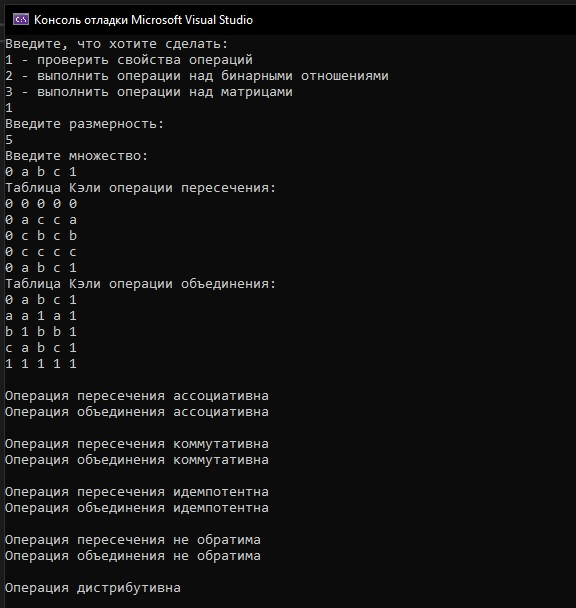
\includegraphics[width=0.9\textwidth]{test_1}
		\caption{Тестировние №1}
		\label{fig:test_1}
	\end{figure}
	
	Тестирование №2:
	
Операция объединения над бинарными отношениями.
	
	\begin{figure}[H]
		\centering
		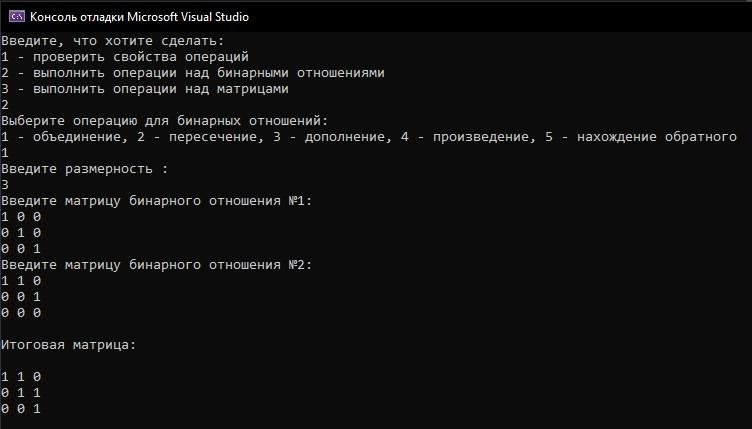
\includegraphics[width=0.9\textwidth]{test_2}
		\caption{Тестировние №2}
		\label{fig:test_2}
	\end{figure}
	
	Тестирование №3:

Операция пересечения над бинарными отношениями.

	
	\begin{figure}[H]
		\centering
		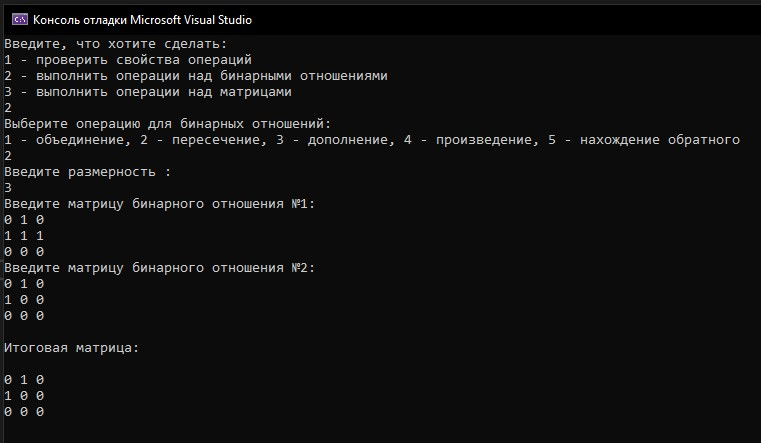
\includegraphics[width=0.9\textwidth]{test_3}
		\caption{Тестировние №3}
		\label{fig:test_3}
	\end{figure}
	
		Тестирование №4:
	
Операция дополнения над бинарным отношением.
	
	
	\begin{figure}[H]
		\centering
		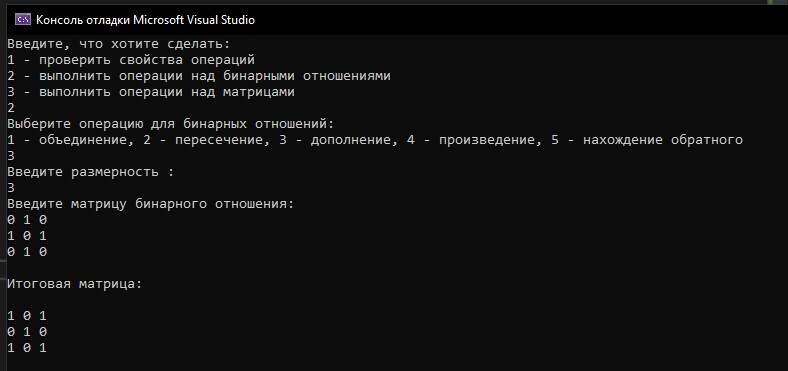
\includegraphics[width=0.9\textwidth]{test_4}
		\caption{Тестировние №4}
		\label{fig:test_4}
	\end{figure}

	Тестирование №5:

Операция произведения над бинарными отношениями.


\begin{figure}[H]
	\centering
	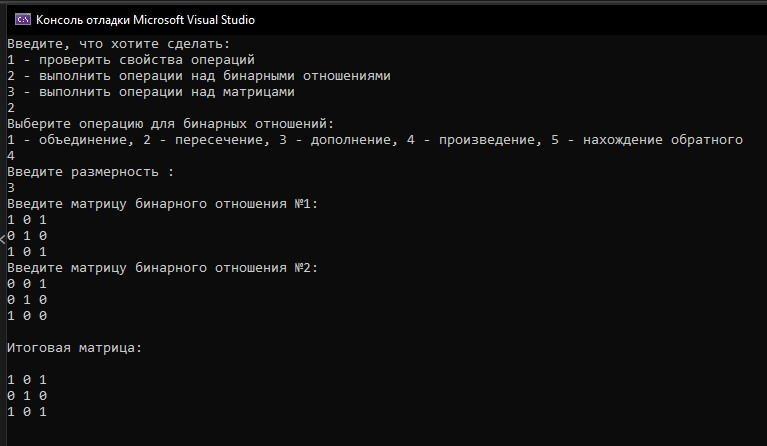
\includegraphics[width=0.9\textwidth]{test_5}
	\caption{Тестировние №5}
	\label{fig:test_5}
\end{figure}

	Тестирование №6:

Операция нахождения обратного над бинарным отношением.


\begin{figure}[H]
	\centering
	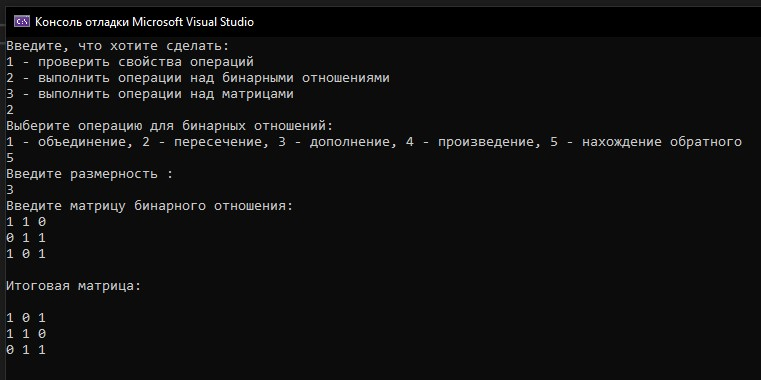
\includegraphics[width=0.9\textwidth]{test_6}
	\caption{Тестировние №6}
	\label{fig:test_6}
\end{figure}

	Тестирование №7:

Операция сложения над матрицами.


\begin{figure}[H]
	\centering
	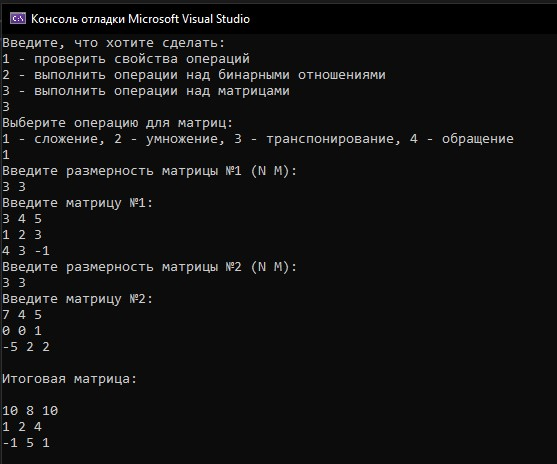
\includegraphics[width=0.9\textwidth]{test_7}
	\caption{Тестировние №7}
	\label{fig:test_7}
\end{figure}

	Тестирование №8:

Операция умножения над матрицами.


\begin{figure}[H]
	\centering
	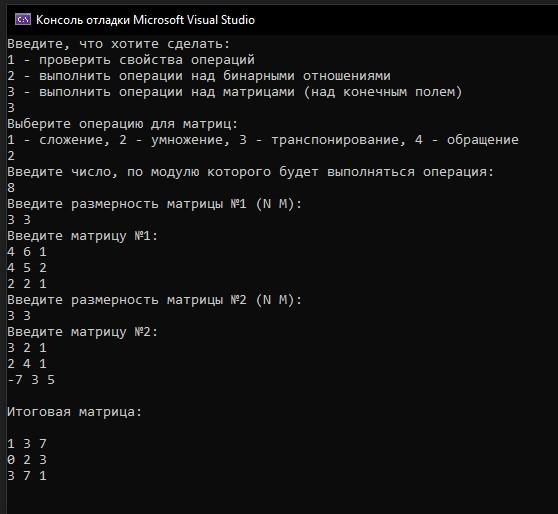
\includegraphics[width=0.9\textwidth]{test_8}
	\caption{Тестировние №8}
	\label{fig:test_8}
\end{figure}

	Тестирование №9:

Операция транспонирования над матрицей.


\begin{figure}[H]
	\centering
	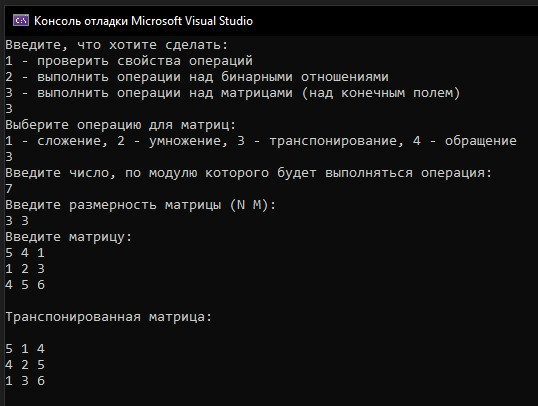
\includegraphics[width=0.9\textwidth]{test_9}
	\caption{Тестировние №9}
	\label{fig:test_9}
\end{figure}

	Тестирование №10:


Операция обращения над матрицей.

\begin{figure}[H]
	\centering
	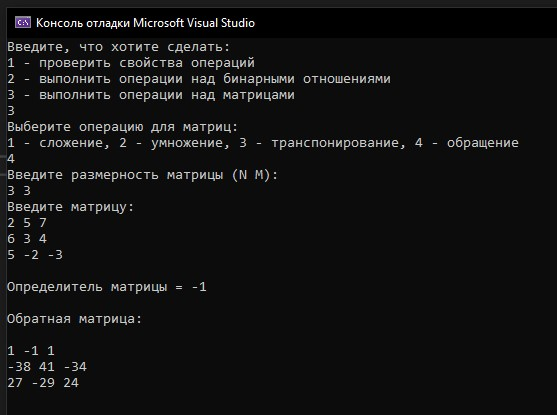
\includegraphics[width=0.9\textwidth]{test_10}
	\caption{Тестировние №10}
	\label{fig:test_10}
\end{figure}
	\newpage
	\conclusion %заключение
	
	В данной лабораторной работе были рассмотрены и изучены следующие темы: понятие алгебраической операции и классификация свойств операций, основные операции над бинарными отношениями и основные операции над матрицами. В третьей части работы были реализованы алгоритмы проверки свойств операций: ассоциативность, коммутативность, идемпотентность, обратимость, дистрибутивность, алгоритмы выполнения операции над бинарными отношениями и алгоритмы выполнения операций над матрицами.  
	  
	
	
	
\end{document}